% vim: tw=80

\chapter{Experimental Setup}
\label{sec:experimental_setup}

The European Organization for Nuclear Research (\CERN) was founded in 1954.
Originally dedicated to the study of atomic nuclei, it is now devoted to the
research of sub-atomic particles and their interactions. To accomplish that
task, \CERN built several particle accelerators reaching record-breaking
energies and explored energy ranges which had not been accessible before.

Ground-breaking achievements like the discovery of neutral currents in the
Gargamelle bubble chamber~\cite{Hasert:1973ff}, the discovery of the W and Z
boson by the UA1 and UA2 experiments~\cite{Arnison:1983rp} at the SPS
accelerator or the creation of antihydrogen atoms were accomplished by physicists at
\CERN.

Remarkable insights into the Standard Model were gained by measurements at
subsequent collider experiments. The mass of the Z and W~boson were precisely
measured at the LEP collider. The proton-antiproton collider Tevatron at FNAL
discovered the top quark and measured its mass accurately. Since the search
for the long anticipated Higgs boson was unsuccesful due to their limited energy
reach, an even larger and more powerful accelerator was planned and built, the
Large Hadron Collider (LHC). The search for the Higgs boson finally succeded in
2012~\cite{Chatrchyan:2012xdj,Aad:2012tfa}, but many further questions like the
nature of dark matter or the existence of supersymmetry are yet to be resolved.

\section{The Large Hadron Collider}

The LHC is the world's most powerful particle accelerator and collider. It
is contained in the circular tunnel of the preceding LEP collider which has a
circumference of \SI{27}{\kilo \meter} at a depth between \SI{50}{\meter} and
\SI{175}{\meter}.  The tunnel crosses the border between Switzerland and France
at four points and two of the four main experiments are located in France. 

Two adjacent beamlines that intersect at four interaction points contain the
particle beams travelling in opposite directions. More than 1000 dipole magnets
generating a magnetic field of up to \SI{8.3}{\tesla} bend the beams on
a circular track while almost 400 quadrupole magnets keep the beams focused. 

The beams are brought to collision at four interaction points which house the
LHC experiments ALICE~\cite{ALICE}, ATLAS~\cite{ATLASa},
\CMS~\cite{Bayatian:922757,Ball:2007zza,Chatrchyan:2008aa} and
\textsc{LHCb}~\cite{LHCb}. ALICE is designed to study the quark-gluon plasma
produced by colliding heavy ions, which resembles the initial state of the
universe. \textsc{LHCb} is precisely measuring the CP violation and the decay of B
mesons. ATLAS and CMS, general purpose detectors which allow a broad field of
physics studies, were built to search and study the Higgs boson and physics
models beyond the Standard Model. Furthermore, precision measurements of
Standard Model predictions and its parameters improve the current knowledge and
confidence in its predictions.

Prior to injection and acceleration of protons in the LHC, the particles pass a
series of consecutive acceleration steps, succesively increasing their energy.
The linear particle accelerator (LINAC2) generates \SI{50}{\mega \electronvolt}
protons that are further accelerated in the Proton Synchrotron Booster (PSB) and
the Proton-Synchrotron (PS) to \SI{26}{\giga \electronvolt}. The
Super-Proton-Synchrotron (SPS) further accelerates the protons up to an energy
of \SI{450}{\giga \electronvolt}. At last, the proton beams are injected into
the LHC ring in which they are accelerated up to peak design energy of
\SI{13}{\tera\electronvolt}. All these pre-accelerators are not only used to
feed the LHC, but also serve other physics experiments like the radioactive ion
beam facility ISOLDE, see Fig.~\ref{fig:lhc_complex}.

\begin{figure}[htbp]
    \centering
    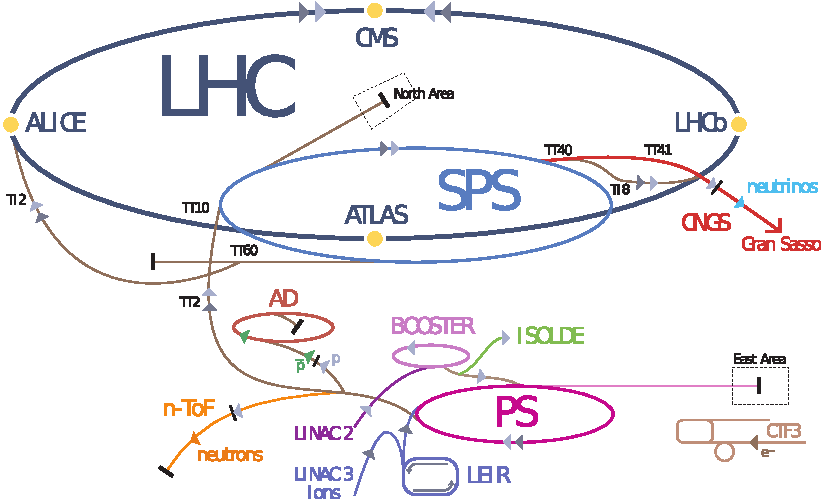
\includegraphics[width=0.8\textwidth]{figures/cms_detector/lhc_accelerator_chain.pdf}
    \caption[\CERN accelerator complex]{Several particle accelerators are
        chained together to feed proton beams into the LHC. Further experiments are
        located along the accelerator complex serving a broad program of physics
        studies~\cite{LHC:COMPLEX}.}
    \label{fig:lhc_complex}
\end{figure}

\section{Luminosity measurement}
\label{sec:lumi_measurement}

The cross section $\sigma$ of a physical process is related to the
event rate $\dot{N}$ by the luminosity~$\mathcal{L}$,

\begin{equation*}
    \dot{N} = \mathcal{L} \sigma.
\end{equation*}

The luminosity is dependent on the particle beam parameters and can be expressed
by

\begin{equation*}
    \mathcal{L} = \frac{n_p^2
        n_b f_\mathrm{rev} \gamma F}{4 \pi \epsilon_n \beta^*},
\end{equation*}

where $n_p$ is the number of particles per bunch, $n_b$ is the number of bunches
per beam, $f_\mathrm{rev}$ the revolution frequency, $\gamma$ the relativistic
gamma factor and $F$ the geometric luminosity reduction factor. The effective
collision area of the two beams is related to the normalized transverse beam
emittance $\epsilon_n$ and the value of the betatron function $\beta^*$ at the
interaction point.
\todo{besser erklaeren}

The instantaneous luminosity is constantly monitored by the experiments. CMS
employs two methods to estimate the relative instantaneous
luminosity~\cite{CMS-PAS-LUM-13-001}. The first method measures the particle
flux in the hadron forward calorimeter which is related to the instantaneous
luminosity. The second counts the number of clusters in the pixel tracking
detector measured in zero-bias events. The absolute luminosity measurement is
relying on van-der-Meer scans carried out in special runs of the
LHC~\cite{vanderMeer:296752}. The luminosity measurement is affected by an
uncertainty, which propagates on any absolute cross section measurement, see
Sec.~\ref{sec:luminosity_uncertainty}.

Fig.~\ref{fig:cms:lumi_integrated} shows the integrated luminosity delivered by
the LHC to the CMS experiment in the run periods from 2010 to 2012.

\begin{figure}[htp]
    \centering
    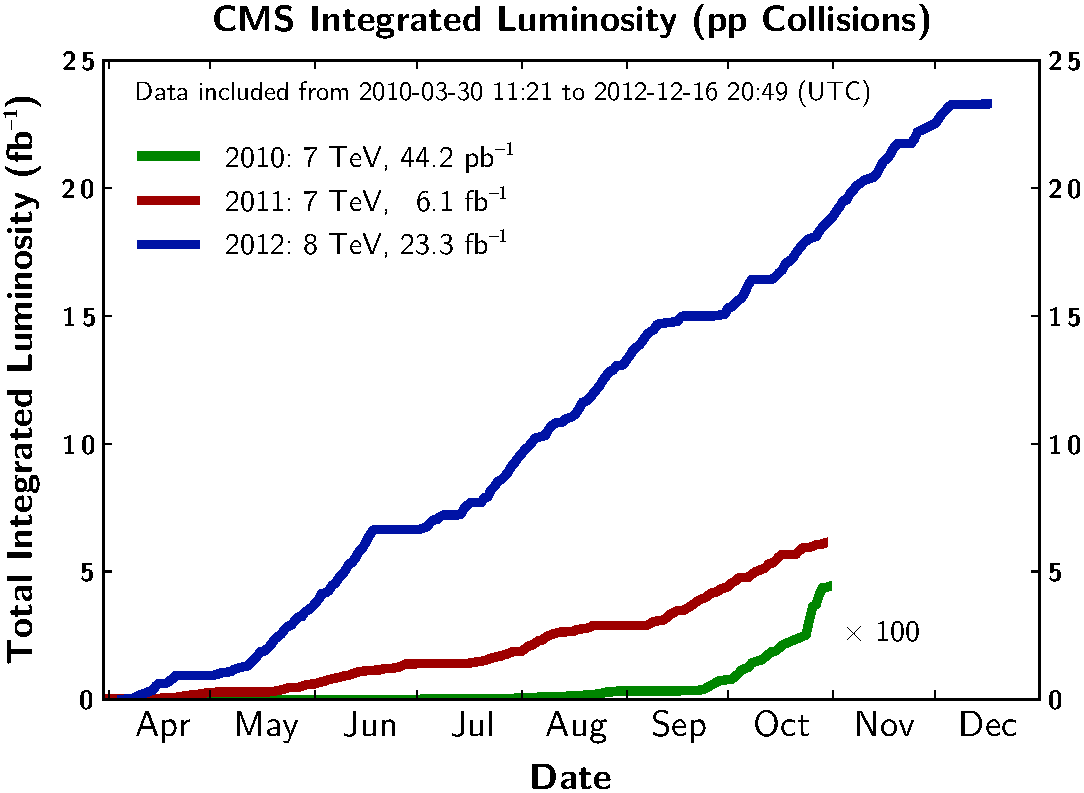
\includegraphics[width=0.9\textwidth]{figures/cms_detector/lumi_integrated.pdf}
    \caption[Integrated luminosity delivered to CMS]{Integrated luminosity
        delivered by the LHC to CMS in the 2010, 2011 and 2012 LHC run periods.
        Taken from~\cite{Berger:2014aca}.}
    \label{fig:cms:lumi_integrated}
\end{figure}


\section{The Compact Muon Solenoid Detector}

The Compact Muon Solenoid (CMS) detector is a general purpose detector at the
LHC, located at Point 5 of the LHC ring. To serve a wide range of physics
studies, the detector design is driven by a cylinder-shaped structure containing
layers of different subdetectors, each built to measure a specific type of
particles with best precision, see Fig.~\ref{fig:cms:transverse_slice}. A
high-precision inner tracking system is surrounded by an electromagnetic and a
hadronic calorimeter which again are enclosed by a superconducting solenoid
magnet. The whole inner part of the detector is surrounded by a sophisticated
muon detection system embedded in an iron yoke.
\todo{vor/nachteile des designs}

\begin{figure}[htp]
    \centering
    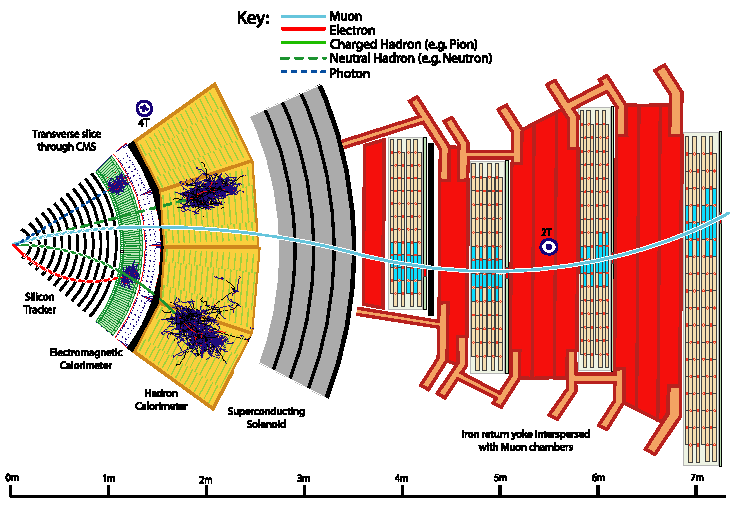
\includegraphics[width=0.9\textwidth]{figures/cms_detector/cms_slice.pdf}
    \caption[Transverse slice of the CMS detector]{A transverse slice through the
        CMS detector shows the various subdetectors and the signatures by which
        passing particles are detected. Taken from~\cite{Barney:2120661}.}
    \label{fig:cms:transverse_slice}
\end{figure}

The detector is \SI{21.6}{\meter} long and \SI{14.6}{\meter} in diameter, but
weighs more than \SI{12000}{\tonne} due to its compact design. It was
constructed as cylyndrical slices constructed at ground level and lowered into
the cavern. In case of upgrades or repairs, the slices can be pulled apart and
the inner components can be easily accessed. A longitudinal section of one
quadrant of the CMS detector, which reveals the location and coverage of all
subdetectors, is shown in Fig.~\ref{fig:cms:longitudinal_section}.

The detector and physics performance of the CMS detector are discussed in great
detail in~\cite{Bayatian:922757,Ball:2007zza,Chatrchyan:2008aa}. This section
intends to only present a short overview of the design and functional principles
of the detector.

\begin{figure}[htp]
    \centering
    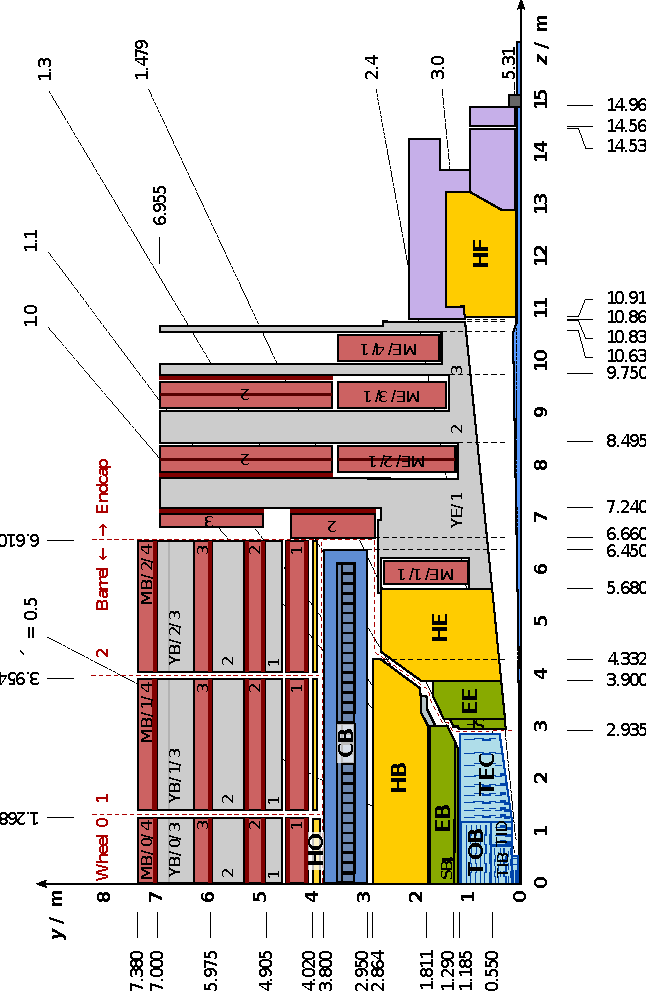
\includegraphics[width=1.0\textwidth]{figures/cms_detector/cms_longitudinal_section.pdf}
    \caption[Longitudinal section of the CMS
    detector]{A longitudinal section of one quadrant of the CMS
        detector in the $y$-$z$ plane. The sketch shows
    the multi-layer design of the CMS detector starting with the silicon pixel
and silicon strip detectors close to the interaction point. They are surrounded
by the electromagnetic (green) and hadronic (yellow) calorimeters. The barrel is
encompassed by the superconducting magnet (blue). The muon detection system
(red) is embedded in the iron return yoke~\cite{Berger:2014aca}.}
    \label{fig:cms:longitudinal_section}
\end{figure}

\subsection{Definition of the Coordinate System}
\label{sec:coord_system}

CMS uses a right-handed coordinate system centered at the nominal interaction point inside the
detector. The $x$-axis points radially inward towards center of the LHC ring, the
$y$-axis vertically upwards and the $z$-axis along the beam direction towards
the Jura mountains. Important quantities are the azimuthal angle $\phi$,
measured from the $x$-axis in the $x$-$y$ plane, and the polar angle $\theta$,
measured from the $z$-axis in the $z$-$y$ plane. Instead of the polar angle
$\theta$, the pseudo-rapidity $\eta$ and the rapidity $y$ are commonly used to
divide the phasespace. The pseudo-rapidity is defined as

\begin{equation*}
    \eta = - \ln \left( \tan \left( \frac{\theta}{2} \right) \right).
\end{equation*}

Throughout this thesis, the rapidity is favored compared to the pseudo-rapidity
due to its invariance under longitudinal boosts in $z$-direction. Rapidity
and pseudo-rapidity are equivalent in case of massless particles. The
rapidity is defined as

\begin{equation*}
    y = \frac{1}{2} \ln \left( \frac{E + p_z}{E - p_z} \right).
\end{equation*}

The momentum along the beamline is not well-defined due to the momentum
distribution inside the proton. A direct connection to the hard process is given
by the transverse momentum \pt related to cartesian coordinates as

\begin{equation*}
    \pt = \sqrt{p_x^2 + p_y^2}.
\end{equation*}

\subsection{Inner Tracking System}

In order to yield a best possible spatial resolution, the particle tracks need to be
measured as close to the beam line as possible. The inner tracking system of CMS
consists of silicon detectors which measure the hits of charged
particles emerging from the collision. 

The silicon detectors are depleted from free charged by applying a voltage. When
charged particles pass through the detector material, they leave a small
ionization current which can be detected and measured as a hit in the detector.
By combining multiple hits, the track of a charged particle can be reconstructed
and the momentum and charge of the particle can be determined based on a mass
hypothesis. Due to the strong magnetic field of the CMS detector, even tracks of
particles with high transverse momenta have a measurable curvature.
 
The inner tracking detector encloses the interaction point with a diameter of
\SI{2.6}{\meter} and extends up to \SI{2.8}{\meter} in each direction along the
beampipe, the tracking system covers a pseudo-rapidity range up to $|\eta| <
2.4$. The inner tracking system comprises two subsystems, the silicon pixel
detector consisting of three layers which is installed very close to the beam
pipe and the silicon strip detector located further outside with ten strip
layers in the barrel region, see Fig.~\ref{fig:cms:inner_tracking}. 

\paragraph{Silicon Pixel Detector} Containing over \SI{65} milion pixels
arranged in three cylindrical layers at \SI{4}{\centi\meter},
\SI{7}{\centi\meter} and \SI{11}{\centi\meter} distance to the beam pipe, the
pixel detector is able to resolve the tracks of a the huge number of particles.
At LHC design luminosity, about 1000 particles pass the tracking detector on
average per bunch crossing. The size of each pixel is \SI{100}{\micro \meter} x
\SI{150}{\micro \meter} giving an average occupancy of $10^{-4}$ per bunch
crossing. The high spatial resolution achieved by the pixel detector furthermore
allows the identification and measurement of secondary vertices used to identify
long-lived particles.

\paragraph{Silicon Strip Detector} The pixel detector is complemented by a silicon
strip detector. Reduced particle flux further away from the beam pipe eases the identification
of tracks. Cost-efficient silicon strips are employed reaching out to
a radius of \SI{1.3}{\meter}. The strip detector consists of a total of 10 million
detecting strips which are read out by \SI{80000} chips. To avoid any blind
detector area, the strips are are arrangeg overlapping.

\begin{figure}[htp]
    \centering
    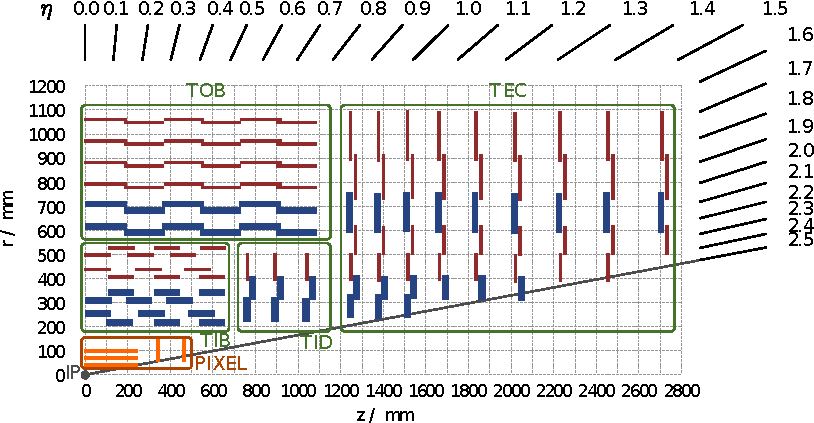
\includegraphics[width=0.65\textwidth]{figures/cms_detector/tracker.pdf}\hfill
    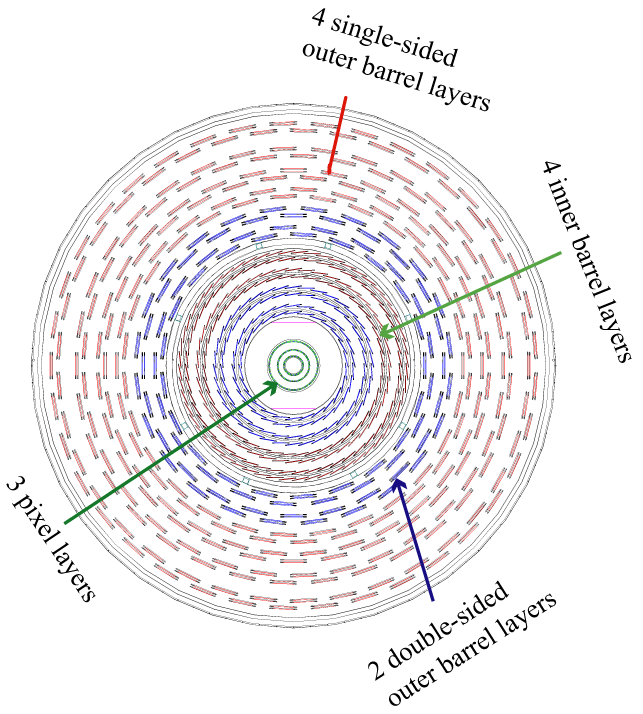
\includegraphics[width=0.3\textwidth]{figures/cms_detector/tracking_sytem_barrel_slice.png}
    \caption[Inner Tracking System]{The left plot shows one quadrant of a
        longitudinal section of the inner tracking system consisting of the
        silicon pixel detector and the silicon strip detector. The right figure shows a
        transverse section of the tracking system in the barrel region which
        nicely illustrates the overlapping arrangement of the strip modules. Figures taken
        from~\cite{Berger:2014aca} and~\cite{cmsweb:innertracker}, respectively.}
    \label{fig:cms:inner_tracking}
\end{figure}

\subsection{Electromagnetic Calorimeter}

Measuring only the tracks of traversing particles is not sufficient to identify
the particles and derive their momentum. The energy needs to be determined as well
by stopping the particles in the detector and summing up the
deposited energy. The photon and electron energy is measured in the
electromagnetic calorimeter (ECAL). 

High-energy photons, electrons or positrons which enter the dense material of
the ECAL detector produce an electromagnetic shower via subsequent
bremsstrahlung and electron-pair production processes. Below a certain
threshold, the particles deposit their energy via compton scattering and the
photoelectric effect in the detector material resulting in an excitation of the
material atomic state. Subsequently, they emit photons which are measured using
avalanche photodiodes. The fraction of the deposited energy is proportional to
the number of emitted photons.

The hermetic calorimeter is made of lead tungstate ($\mathrm{PbWO}_4$), a very
dense material with a radiation length of $X_0 = \SI{0.89}{\centi\meter}$.
Because of the incorporated oxygen, it is highly transparent and scintillates
light. The small Moli\`ere  radius of \SI{2.19}{\centi\meter} leads to a fine
granularity.  These material properties allow the ECAL to be built very compact
and to be placed within the solenoid magnet. 

\begin{figure}[htp]
    \centering
    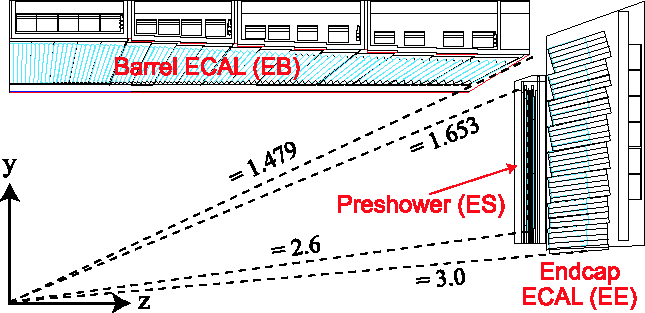
\includegraphics[width=0.8\textwidth]{figures/cms_detector/cms_ecal.pdf}\hfill
    \caption[Electromagnetic Calorimeter]{The electromagnetic calorimeter
    consists of submodules covering the barrel region (EB) and the endcaps (EE).
    A complementary preshower detector (ES) is mounted in front of the
    endcaps. Taken from~\cite{Bayatian:922757}.}
    \label{fig:cms:ecal}
\end{figure}

Figure~\ref{fig:cms:ecal} shows a schematic sketch of the ECAL in the $y$-$z$
plane. The ECAL comprises three subsystems covering the the pseudo-rapidity
range up to 3.0. 

\paragraph{Electromagnetic Calorimeter Barrel (EB)} 
The EB extends up to $\eta < 1.479$ using more than \num{60000} crystals which form a
homogenous coverage in pseudo-rapidity. Each crystal measures
$\SI{2.2}{\centi\meter} \times \SI{2.2}{\centi\meter} \times
\SI{23}{\centi\meter}$ which corresponds to 25.8 $X_0$ radiation lengths.

\paragraph{Electromagnetic Calorimeter Endcaps(EE)} 
The ECAL endcaps seal off the barrel region and extend the pseudo rapidity
coverage in the region $1.479 < |\eta| < 3.0$ with an additional \SI{15000}
crystals.

\paragraph{Electromagnetic Pre-shower Detector (ES)} 
To incrase the spatial precision, the EE is complemented with the ES, which sits
in front of it and consists of two orthogonal silicon strip sensors. The ES
improves the discrimination between single high-energy photons and less
interesting low-energy photon pairs as well as the discrimination between
neutral pions and photons.

The relative energy resolution of the ECAL can be parametrized using the NSC-formula

\begin{equation*}
    \left( \frac{\sigma}{E} \right)^2 = \frac{N^2}{E^2} + \frac{S^2}{E} + C^2,
\end{equation*}

in which the first term describes the contribution by noise (N), the second
term the stochastic (S) component arising from the proportional relation between
the number of counted photons and the deposited energy, and last a constant (C)
offset term.
\todo{add resolution values}

\subsection{Hadronic Calorimeter}

Hadrons entering the calorimeter produce hadronic showers. High-energy
hadrons mostly shower in inelastic interactions producing a large number of pions
and nucleons. Due to the large transverse momentum of the secondary particles,
hadronic showers spread further in the calorimeter than electromagnetic showers.
When the energy of the particles involved in the shower drops below a certain
theshold, the energy is deposited by ionization and low-energy hadronic
activity. The active scintillation material is excited and emits blue-violet
light. All scintillators are connected to photodiodes using wavelength
shifters which read out the signals and pass them to the data aquisition system.

The compact design of the CMS detector limits the size of the calorimeters. CMS
therefore built a sampling calorimeter inside the solenoid coil. The hadronic
calorimeter consists of brass as absorber material because it is is non-magnetic and
has a short interaction length of $\lambda_I = \SI{16}{\centi\metre}$. It is
interleaved with plastic scintillators measuring the deposited energy. The CMS
hadronic calorimeter comprises three subsystems. 

\paragraph{Hadron Barrel Calorimeter (HB)}
It covers the barrel region up to a pseudo-rapidity $|\eta| < 1.305$. The
absorbing material in the barrel has a corresponding thickness of
$\SI{5.39}{\lambda}$ in the central region and up to $\SI{10.3}{\lambda}$ at $|\eta|
= 1.3$. The HB is complemented by the Hadron Outer Calorimeter (HO) located on
top of the coil of the magnet. Using the coil as absorbing material, it is able
to measure the tails of hadron showers penetrating the HB and the coil.

\paragraph{Hadron Endcap Calorimeter (HE)} The HE extends the pseudo-rapidity
coverage up to $|\eta| < 3.0$. A major challenge in the construction of the HE
were the usage of non-magnetic material in order to not disturb the magnetic field as
well as the close distance to the beampipe. Radiation damages decrease the
detector response which has to be corrected continuously. 

\paragraph{Hadron Forward Calorimeter (HF)} 
The forward calorimeter extends even closer to the beam pipe. With a coverage of
$2.8 < |\eta| < 5.2$ the calorimeter is adapted to the high radiation
environment. The HF is built using iron absorbers and quartz fibres as active
material, which measure the Cerenkov light emitted by the relativistic
components of the shower.
\todo{add resolution}

\subsection{Superconducting Solenoid}

A key component of the CMS detector is the superconducting magnet which
produces a magnetic field with a strength of \SI{4}{\tesla} and is located
inside the detector between the calorimeters and the muon system. It measures a
diameter of \SI{6}{\meter} and a length of \SI{12.5}{\meter}. When operated at
design magnetic field strength, the magnet contains an energy of
\SI{2.6}{\giga\joule}. The strong magnetic field is neccessary to bend the
tracks of particles with high momentum to achieve a good resolution in the
tracking system. Operated at a temperature of \SI{4}{\kelvin}, the NbTi conductors become
superconducting. The magnet is complemented by a \SI{10000}{\tonne} iron yoke
which returns the magnetic field.

\subsection{Muon System}

Identifying and measuring muons with high precision is an unrivaled capacity of
the CMS detector. Unlike most other particles, muons are not stopped by the
calorimeters but leave the detector. Therefore, the muon system has been placed
around the other detector components in the iron return yoke of the magnet to
measure the bended tracks of the muons.

By combining the information of the inner tracking system and the muon
detectors, the path and the muon momentum are both measured precisely. The muon
system comprises three different types of detectors each suited for a specific
task. Drift tubes (DT) cover the barrel region up to $|\eta| < 1.2$, the endcaps
up to $|\eta| < 2.4$ contain cathode strip chambers (CSC) which also
work reliably in spatially varying magnetic field. The DT and CSC detectors
yield a precise spatial muon resolution. Both systems are accompanied by
resistive plate chambers (RPC) which provide fast response to the trigger
system.

\subsection{Trigger and Data Aquisition at CMS}

The LHC generates a huge number of collisions. At beam crossing frequencies of
\SI{25}{\nano \second}, there are 40 million bunch crossings per second with an
average of around 20 collisions per bunch crossing in the 2012 run period. With
today's hardware, the storage of all collision events is not feasible.
Furthermore, most of the collisions are soft and of low interest for physics
analyses. Therefore, a complex trigger system consisting of a very fast
component implemented in hardware, the Level 1 trigger (L1) and a High Level
software trigger (HLT) analyze the events and accept only events which are
interesting for physics analyses.

\begin{figure}[htp]
    \centering
    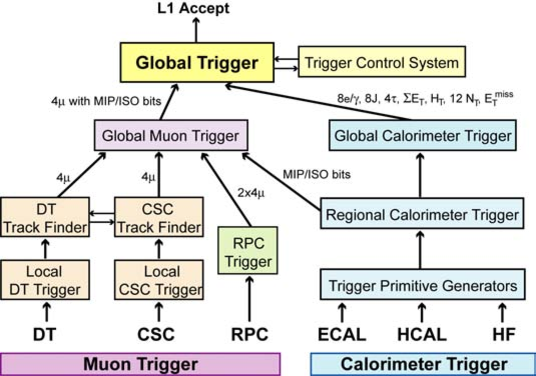
\includegraphics[width=0.8\textwidth]{figures/cms_detector/cms_l1_trigger_new.pdf}\hfill
    \caption[The L1 Trigger of CMS]{Workflow of the L1 trigger system. The
        regional triggers search for jets and compute the transverse and missing
        energy of an event. The global calorimeter trigger sorts the objects
        from the regional calorimeter triggers and passes the top candidates to
        the Global trigger, which accepts or rejects the event. If it is
        accepted, the complete data and the trigger objects are passed to the
        DAQ. Taken from~\cite{Bayatian:922757}.} 
    \label{fig:cms:l1_trigger}
\end{figure}

\paragraph{L1 Trigger} 
At the same frequency as collisions occur, the L1 trigger reads out the detector
electronics and analyzes the data using custom hardware. The workflow of the L1
trigger is shown in Fig.~\ref{fig:cms:l1_trigger}. Trigger Primitive Generators
calculate the transverse energy and missing energy from the front-end electronics
readout. Regional Calorimeter Triggers (RCT) identify electromagnetic showers
in the ECAL and sum up ECAL and HCAL trigger towers. Furthermore, pattern
recognition is performed to identify jets and hadronic $\tau$ decays. A jet
candidate is found, if the transverse energy in a region of $4\times4$ trigger
towers is greater as or equal to the transverse energy of the eight surrounding
regions, see Fig.~\ref{fig:cms:l1_calo_towers}. These
candidates are passed to the Global Calorimeter Trigger (GCT), which sorts the
incoming candidates from all 18 regional triggers and passes the top
candidates to the Global Trigger (GT). The GT accepts events with a frequency
of \SI{100}{\kilo\hertz} and passes them to the data aquisition system, which
processes the data and transfers them to the HLT.

\begin{figure}[htp]
    \centering
    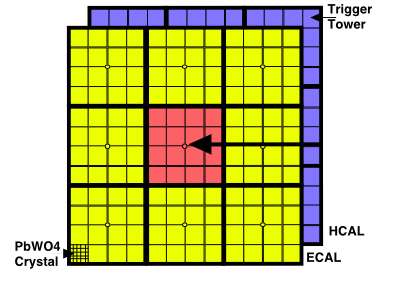
\includegraphics[width=0.8\textwidth]{figures/cms_detector/l1_calo_towers.png}\hfill
    \caption[Jet Candidates in the Level 1 calorimeter trigger]{Jet Candidates
        in the Level 1 calorimeter trigger are formed from $4\times4$ trigger
        towers. Taken from~\cite{Rose:2009zz}.}
    \label{fig:cms:l1_calo_towers}
\end{figure}

\paragraph{HLT Trigger} 
The HLT is a software-based trigger running on a dedicated computing farm at
Point 5. The software is implemented in a streamlined version of the CMS
software framework. Each HLT path is a sequence of reconstruction and
selection steps with increasing complexity. In the end, the HLT accepts several
100 events per second for permanent storage and analysis.

Jets are reconstructed in the HLT using the \antikt jet clustering algorithm. Because of the
high processing time of the Particle Flow algorithm, see
Sec.~\ref{sec:particle_flow_algorithm}, the jet trigger paths are divided into
multiple selection steps. At first, jets are reconstructed from calorimeter
towers.  Only for events in which at least one calorimeter jet passes a certain
\pt threshold, the Particle Flow algorithm is run and the jets are clustered
again from the Particle Flow candidates. Due to the flexibility of the HLT, it
is already possible to apply sophisticated jet energy corrections during the HLT
 selection.

\paragraph{Data Aquisition (DAQ)}

As the L1 trigger accepts events at a rate of \SI{100}{\kilo\hertz}, the DAQ
system has to process the events at the same speed. It reads out the data of all
detector subcomponents and assembles the complete events, see
Fig.~\ref{fig:cms:daq_system}. The data is subsequently passed to the HLT  which
further reduces the rates to a few hundred events per second. Finally, the events are
merged and saved to a local storage system, from which they are continuously
transferred to the Tier-0 computing center at \CERN.

\begin{figure}[h!tp]
    \centering
    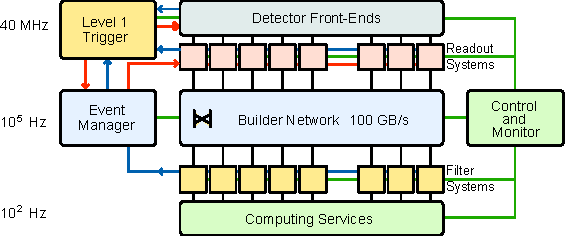
\includegraphics[width=0.8\textwidth]{figures/cms_detector/cms_daq_new.pdf}\hfill
    \caption[The DAQ System of CMS]{The L1 trigger accepts events at a rate of
        \SI{100}{\kilo\hertz} and passes them to the DAQ. The DAQ reads out
        all detector signals, builds the complete event and passes it to the
        HLT. All events accepted by the HLT are stored and transferred to the
        Tier-0 computing center. Taken from~\cite{Bayatian:922757}.}
    \label{fig:cms:daq_system}
\end{figure}

\section{Computing Infrastructure and Software Tools}

The vast amount of data produced at the LHC experiments and the complexity of
the software pose many challenges for the computing infrastructure and the
engaged software. On the theory side, powerful Monte-Carlo event generators,
which are able to simulate the collision events need to be developed. On
experimental side, the physical event information needs to be reconstructed from
the raw detector readout. Furthermore, the complex architecture of the detector
response needs to be modelled and simulated. These central tasks are approached
using a common software framework within CMS, the \CMSSW framework, which
interfaces the various theory tools and all the reconstruction and detector
software. All arising processing tasks are divided into smaller units, called
jobs, which are assigned to computing centers distributed over many countries.
This common computing and storage infrastructure is called the worldwide LHC
computing grid (LHCG).

\subsection{Worldwide LHC Computing Grid}

To overcome the discussed challenges and to ease the access of users to the data of
the LHC experiments, a distributed grid with a tiered infrastructure was
developed. As the majority of the data is produced at \CERN, a hierarchical
structure with the computing center at \CERN at the top was
chosen, see Fig.~\ref{fig:lhc_tier_structure}. The raw data is stored at \CERN
and distributed to globally distributed Tier-1 centers, as they provide further
storage resources and large computing resources for the reconstruction and
analysis of the data. Tier-2 sites provide additional computing ressources while
Tier-3 sites are mostly used by local groups for data analysis.

\begin{figure}[htp]
    \centering
    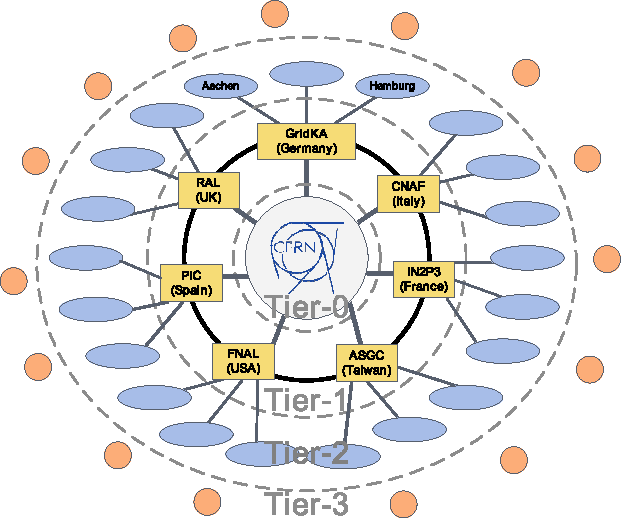
\includegraphics[width=0.8\textwidth]{figures/cms_detector/lhcg.pdf}\hfill
    \caption[Tiered structure of the worldwide LHC Computing Grid]{The Worldwide
        LHC Computing Grid is ordered hierarchically with the \CERN Tier-T0 at the top. Taken
        from~\cite{Stober:2012abc}.}
    \label{fig:lhc_tier_structure}
\end{figure}

Access to the resources of the LHCG is gained by certificates which authorize
the user to access the storage and computing resources.


\subsection{CMS Software Framework}

The software framework of the CMS collaboration (\CMSSW)~\cite{Bayatyan:838359}, offers
all neccessary tools for a physics analysis. The tasks in the event processing
comprise on the one hand calibration and reconstruction of data from raw
detector read-out and on the other hand the event generation and detector
simulation. Furthermore, it provides the possibility to implement analysis code
to perform the data analysis. 

To cope with this vast range of requirements to the experiment software, \CMSSW
is built on top of an event data model (EDM), in which the event is a
container for all measured or simulated data. The reconstruction and
distribution algorithms in \CMSSW are divided into modules, which can be
dynamically loaded and run. Each module reads the event data and can add additional
objects to the event. The execution of modules is ordered
in processing chains which can be configured by the user. Very often these modules
access external libraries like Monte Carlo event generators for event
simulation, Geant 4 for the detector simulation or FastJet for the
reconstruction of jets. 

While having that much information in the event data is convenient to redo
reconstruction steps, it is unsuited for fast processing in the analysis due to
its size and complexity. Therefore a skimming step, in which only the neccesary
data is preserved is run before the analysis, see Section~\ref{artus_kappa}.

\subsection{Analysis Software and Workflow}

Due to the complexity of the workflows in the HEP data analysis, several
analysis tools were used or even deloped in the Karlsruhe group to faciliate a reliable and
fast workflow of the analysis. 

\subsubsection{Artus and Kappa}
\label{artus_kappa}

The Kappa software~\cite{Kappa:2015aa} is a skimming framework interfaced to
\CMSSW. It consists of different modules which allow to skim only the physics
objects needed in the subsequent analysis. The data is stored in its distinct
compact data format using the ROOT object serialization capabilities. The
resulting Kappa tuples provide all neccesary information of the events and the
lumisections, while hiding the complexity of the \CMSSW datasets.

\begin{figure}[htp]
    \centering
    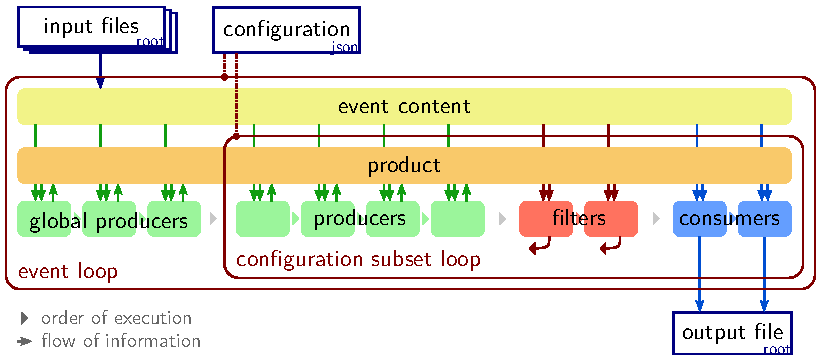
\includegraphics[width=0.8\textwidth]{figures/cms_detector/artus_workflow.pdf}
    \caption[Workflow of an analysis in the Artus framework]{Workflow of an
        analysis in the Artus analysis framework. Taken
        from~\cite{Berger:2014aca}.}
    \label{fig:artus_workflow}
\end{figure}

The analysis itself is built on top of the Artus framework~\cite{Berger:2015qao}.
Artus has been developed within the Karlsruhe group to combine analysis efforts
and to profit from mutual developments. The framework defines a workflow based
on three elements, see Fig.~\ref{fig:artus_workflow}. There are
\emph{producers}, which calculate quantities and \emph{filters}, which reject
events based on the defined criteria. In a final step, histograms or tuples are
written out by \emph{consumers}. All producers, filters and consumers are
written in a modular way so that they can be shared with other analyses.
Furthermore they are steered by a global configuration file in which all
settings and cuts can be easily adapted.

\subsubsection{grid-control}

The data sets are even after the skimming step too large to be processed on a
single computer. Therefore special batch systems with a large number of
computing nodes are employed to process the data. The data processing is split
into multiple jobs which are then sent to the batch system.
grid-control~\cite{Gridcontrol:2015aa} is by far the most versatile job
submission tool which provides multiple options for data splitting and
parametrized jobs while hiding the pitfalls of local or remote computing
resources.

\subsubsection{ROOT}

The object-oriented data analysis framework ROOT~\cite{Brun:1997pa} has been
written more than 20 years ago. However it is still very popular and used by all
LHC experiments for persistent storage of data. Moreover, ROOT provides fast
histogramming classes and access to many libraries like MINUIT for minimization
purposes or TMVA for multivariate data analyses. Despite many hours of headaches
caused by obscure design decisions in the software, ROOT and especially the
python bindings \textsc{PyROOT} are used extensively in this analysis.

\subsubsection{matplotlib and numpy}

matplotlib is a 2D plotting library written in the python programming language~\cite{Hunter:2007aa}. It
provides publication quality plots in a variety of output formats and is very
pleasant to use. All plots in this thesis were made using matplotlib. The
plotting library matplotlib as well as many scripts used in this thesis rely on
the scientific computing library NumPy~\cite{Oliphant:2007aa}. NumPy provides
powerful n-dimensional arrays and tools to manipulate them. 

\subsection{Monte-Carlo Event Generators and Simulation Software}
\label{subsection:mc_generators}

\subsubsection{Pythia}

The multi-purpose event generator Pythia simulates events in high-energy
collisons, comprising a large set of physics processes. Pythia uses the Lund
string hadronization model in which all but the highest-energy gluons are
treated as field ines which attract each other by gluon self-interaction and
form a tube or string of strong color field. In this analysis two version of the
Pythia event generator are used. The official samples including the detector
simulation were generated using Madgraph and Pythia~6~\cite{Sjostrand:2006za},
while the study of non-perturbative effects was performed using the new
Pythia~8~\cite{Sjostrand:2007gs} version, in which all the employed tunes are
available. 

\subsubsection{Herwig}

Herwig is also a multi purpose event generator for the simulation of high-energy
hadron-hadron collisions. The first version was build in Fortran and is known as
HERWIG~\cite{Corcella:2000bw}. Herwig++~\cite{Bahr:2008pv} builds up on the
heritage of the HERWIG version while providing a much more flexible structure as
it is implemented in C++. The recently released Herwig~7~\cite{Bellm:2015jjp}
version combines all their developments and supersedes both version. 

The Herwig generator family includes all steps to simulate events. It includes a
number of hard scattering processes, but also possesses the possibility to
interface external matrix element generators. The parton shower simulates
initial- and final-state radiation via angular ordering, multiple partonic
scatterings are simulated by an eikonal model and a cluster model decribes the
hadronization. 

Herwig 7 further improves these capabilities by including next-to-leading order
QCD matrix elements with matched parton showers while keeping the key features
of the previous Herwig versions. Herwig++ is used in this thesis to study
non-perturbative effects, see Sec.~\ref{sec:np_factors}. The NLO capabilities of
Herwig 7 are shown in the comparison of the unfolded measurement to NLO
predictions with matched parton showers, see Sec.~\ref{sec:nlo_comparisons}.

\subsubsection{MadGraph}

MadGraph~\cite{Alwall:2011uj} is an automated multi-purpose tree-element matrix
element generator. It implements a large number of processes and can be
interfaced to Monte Carlo Event generators. In this thesis the MadGraph matrix
elements are used together with the Pythia 6 event generator for general
comparisons to data.

\subsubsection{NLOJet++ and fastNLO}
\label{sec:nlojetpp}

The complicated NLO cross section for jet productions are calculated using
\NLOJETPP~\cite{Nagy:2003tz}. It implements the dipole subtraction method for
the separation of the divergences. \NLOJETPP can calulate up to three-jet
observables at NLO precision. It implements the ability run analysis scenarios
by which it is interfaced to \fastNLO~\cite{Kluge:2006xs,Britzger:2012bs}.

Since the pQCD cross section calculations in \NLOJETPP are determined in Monte
Carlo integration and are therefore very time consuming, it is not feasible to
repeatedly calculate the cross sections as it is neccessary for PDF fits or
uncertainty estimations. The \fastNLO framework implements a strategy for fast
recalculations of cross sections. It stores the perturbative coefficients
obtained with \NLOJETPP in a way that the strong coupling constant and the PDFs
can be changed afterwards without a recalculation of the perturbative
coefficients.

\subsubsection{LHAPDF}

All event generators and cross section calculation tools need the parton
distribution functions as input. They are either hardcoded in the generator or
accessed using a standardized interface, the LHAPDF
library~\cite{Whalley:2005nh,Buckley:2014ana}. LHAPDF stores the PDFs in a discritized
structure in data files. It provides interpolation routines to read the PDFs and
interpolate the PDFs at all scales. LHAPDF is used by almost all major MC
generators.


\section{Reconstruction of Jets}
\label{sec:jet_reconstruction}

In scattering processes with large momentum transfers, the outgoing partons
produce a collimated stream of particles when hadronizing. The clusters of these
particles are the experimental signatures of quarks and gluons in the detector
and are called \emph{jets}. The clustering of the particles is performed using
jet algorithms, which are discussed in Sec.~\ref{sec:jet_algorithms}. An
important property of jet algorithms is their applicability to all kinds of
input objects, \ie partons, stable particles or reconstructed particle
candidates. Consequently, the clustered jets are called parton jets, particle
jets, and reconstructed jets, respectively\footnote{In analogy, the 
corresponding levels are later referred to as parton level, particle level
and reconstructed level.}. Fig.~\ref{fig:jet_levels} illustrates the different
levels, at which jets can be clustered.

In the \CMS detector, jets show up as localized deposit of energy in the
calorimeters accompanied by a large number of tracks in the direction of the
deposited energy. The particle candidates, input of the jet algorithm,  are
reconstructed using different techniques based on the amount of information
available. If jets are reconstructed from the energy clusters within the
calorimeters, they are called \emph{calorimeter jets}. If the jet reconstruction
uses Particle Flow candidates, they are called \emph{Particle Flow jets}. By
removing pile-up tracks from the Particle Flow candidates before the jet
clustering, one yields \emph{Particle Flow CHS jets}. 

In the analysis which is presented in this thesis, all jets are clustered using
the anti-\kt algorithm with a jet size parameter of $R=0.7$. When talking about
jets which are clustered at reconstructed level, it is always referred to
Particle Flow CHS jets.

\begin{figure}[h!tbp]
    \centering
    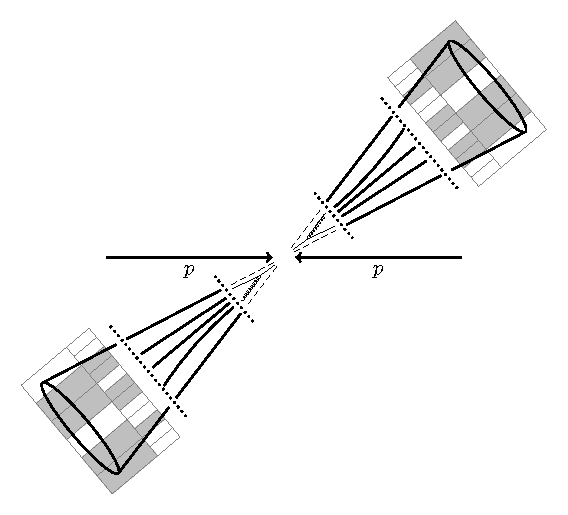
\includegraphics[width=0.7\textwidth]{figures/drawings/particlejet.pdf}
    \caption[Illustration of jet clustering levels]{Illustration of different
    levels at which jets can be clustered. If partons or stable particles are
clustered into yets, parton jets or particle jets are yielded, respectively.
Jets clustered from reconstructed particle candiates are calle reconstructed
jets.}
    \label{fig:jet_levels}
\end{figure}


\subsection{The Particle Flow Algorithm}
\label{sec:particle_flow_algorithm}

\CMS uses the Particle Flow reconstruction
algorithm~\cite{CMS-PAS-PFT-09-001,CMS-PAS-PFT-10-001} to identify and
reconstruct particles by combining information from all detector
subsystems. Due to its compact design inside the solenoid, the hadronic
calorimeter is not able to stop and measure all particles which reduces the
energy resolution. However, taking into account the additional information of
the tracking system within the Particle Flow algorithm enhances the
reconstruction performance and leads to a jet energy resolution comparable to
\ATLAS. A key element in the Particle Flow algorithm is the strong magnetic field
of \CMS which allows the precise distinction between neutral and charged hadrons. 

The ingredients of the Particle Flow algorithm are the
tracks and vertices, reconstructed from hits in the tracking detectors, the
deposited energy in the electromagnetic and hadronic calorimeters and the tracks
in the muon system. The reconstructed particles are classified as muons,
electrons, photons, charged hadrons or neutral hadrons. The combination of all
sub-detectors yields an optimal identification and measurement of their momentum
and energy.

The tracks are found using the Combinatorial Track Finder (CTF)
algorithm~\cite{Adam:2005cg} employed by \CMS. Based on these tracks, the primary
vertices in an event are identified. The electromagnetic and hadronic
calorimeters are divided into a grid of cells based on the detector granularity
to identify calorimeter cluster seeds. If there are seeds with an energy
exceeding a certain threshold, they are used in an iterative merging algorithm
to form Particle Flow clusters. The different elements of the detector
information are then linked together into Particle Flow building blocks based on
the geometry and \chisq fits. At first, muons, which can be well identified
using the tracks in the muon detector, are reconstructed using the building
blocks connected to the muon system. Blocks connecting the inner
tracking system with the ECAL clusters are used to identify electrons.
Similarly, charged hadrons are identified using links between the
tracking system and the remaining calorimeter clusters. Only neutral objects
which leave no traces in the tracking system, remain. ECAL clusters are
interpreted as photon candidates, while the remaining HCAL clusters are assumed
to be deposits of neutral hadrons. To avoid any kind of double-counting of
energy, all Particle Flow building blocks of successfully reconstructed particle
candidates are removed and the energy of the calorimeter clusters is recalculated.

Finally, a set of so-called Particle Flow candidates is yielded. They consist of
well identified particles, which profit from the improved resolution gained by
the inclusion of tracking information. This collection of particles is then
used to reconstruct the jets and further physical objects.

\subsection{Jet Area}

The jet area describes the space covered by a jet object in the $\eta$-$\phi$
plane~\cite{Cacciari:2008gn}. While cone-based jet algorithms yield a $\pi R^2$
size area, the area for sequential jet algorithms needs to be determined for
each jet. A large number of infinitely soft particles, so-called ghost
particles, are evenly distributed in the event. The area $A_j$ of a jet $j$ is
assumed to be proportional to the number of ghost particles clustered into the
jet. 

The concept of jet areas is especially important in the context of pile-up
mitigation. The average \pt density $\rho$ in an event is estimated using the inclusive
\kt algorithm which also clusters many soft jets in the event and covers the
entire $\phi$-$\eta$ phase space. The average \pt density is defined as

\begin{equation*}
    \rho = \text{median} \frac{\pt^j}{A_j}
\end{equation*}

$\rho$ is a measure for the underlying event and pile-up activity in the event
and is used later on to correct the jets for these effects, see
Sec.~\ref{pileup_correction}.

\section{Charged Hadron Subtraction}
\label{sec:chs_algorithm}

\todo[inline]{define primary vertex. something like that: The primary vertex collection
    is sorted according to the sum of the Pt squared of the tracks associated to
    each vertex, such that the vertex with largest sum, likely to be the
    "signal" vertex, appears first. Some justification of this can be found in
the Higgs note CMS-AN-11-129.}

\CMS introduced a new technique to reduce pile-up from jets using the high
resolution of the tracker, called Charged Hadron Subtraction
(CHS)~\cite{Kirschenmann:2014dla}. Naturally the CHS algorithm can only be
applied on jets within the tracker coverage of $|\eta| < 2.4$. All tracks of
Particle Flow candidates which originate from a pile-up vertex are removed, see
Fig.~\ref{fig:chs_jets}. Tracks originating from the main vertex or tracks not
associated with any vertex remain in the event. The jets are clustered from this
set of particles.  Since the jet identification criteria in the jet selection in
the analysis require at least one charged particle in a jet, the CHS method is
effectively reducing the influence of pile-up on real jets as well as completely
removing a majority of the pile-up jets in the barrel region of the \CMS
detector in combination with the jet identification criteria.

The analysis presented in this thesis relies on CHS jets. Especially in the
low-\pt region, removing pile-up jets mimicking the leading jet in the event
improves the signal efficiency in the forward region.

\begin{figure}[h!tbp]
    \centering
    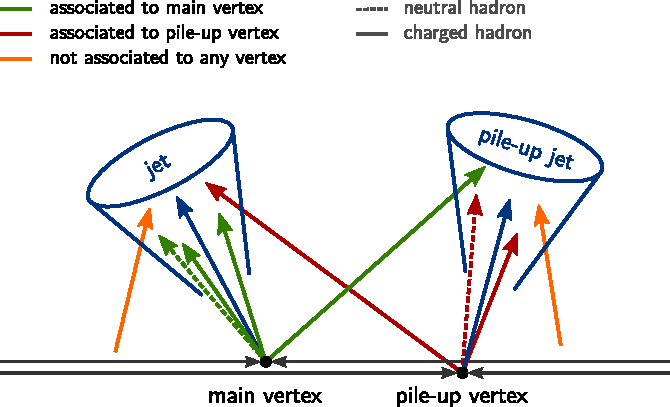
\includegraphics[width=0.95\textwidth]{figures/jet_reconstruction/chs.pdf}
    \caption[Charged Hadron Subtraction]{Illustration of particles clustered
    into a jet which orginates from the main vertex or into a pile-up jet. The
    CHS algorithm removes charged particles not originating from the main vertex
    before clustering the jets.}
    \label{fig:chs_jets}
\end{figure}


\subsection{Jet Energy Corrections}
\label{sec:jec}
\todo{jec paper ref}

A detailed understanding of the jet energy scale and the jet transverse momentum
resolution is important when it comes to drawing conclusions about the
properties of quarks and gluons produced in high-energy scattering processes. On the
experimental side, there are multiple effects causing the reconstructed jet
energy not to correspond to the true jet energy like electronic noise, pile-up
and underlying event effects, but also non-linearities in the calorimeter
response and numerous further small effects. The jet reconstruction and
definition itself also introduces effects due to the fragmentation model,
initial- and final-state radiation which can cause out-of-cone effects.

The jet energy corrections (JEC) relate the measured jet energy to the
corresponding true particle jet energy. \CMS uses a factorized correction approach
consisting of multiple correction steps that build on one another. The corrected
transverse momentum $\pt^{\mathrm{corr}}$ of a jet is yielded by subsequently applying all correction
factors on an uncorrected jet

\begin{equation*}
    \pt^{\mathrm{corr}} = c_{\mathrm{res}} (\eta, \pt^{\prime}) \cdot c_{\mathrm{mc}}
    (\eta, \pt^{\prime\prime}) \cdot c_{\mathrm{pileup}}(\eta, \rho, A_j,
    \pt^{\mathrm{raw}}) \cdot \pt^{\mathrm{raw}},
\end{equation*}

\todo{switch to $p_{\mu}$?}

where $\pt^{\mathrm{raw}}$ is the transverse momentum of the uncorrected jet,
$\pt^{\prime}$ is the transverse momentum after applying the pile-up correction
factor $c_{\mathrm{pileup}}$. $\pt^{\prime\prime}$ is the transverse momentum
after the additional correction $c_\mathrm{MC}$ of relative and absolute effects
derived from MC studies. Finally a correction for residual effects
$c_{\mathrm{res}}$ derived from data is applied to yield the corrected jet
transverse momentum.

\paragraph{Pile-up Corrections}
\label{pileup_correction}

The first step removes the effects of pile-up contamination. Additional soft
proton-proton interactions produce particles being clustered into the jets
originating from the hard interaction. This additional amount of energy needs to
be subtracted by the pile-up correction. The applied correction is based on the
jet area method by using the pile-up density $\rho$ in the event and the jet
area $A_j$. The raw jet energy is then corrected by a factor proportional to the
pile-up density and the jet area.

\paragraph{MC Corrections}

Based on simulated QCD events, the jet energy scale is further corrected. The
momentum of a reconstructed jet can differ from a generated particle jet due to
out-of-cone effects or detector inefficiencies, which are modeled by the detector
simulation. The inverse response of the reconstructed jet to a generated jet is
applied as correction to remove these effects.

\paragraph{Residual Data Corrections}

Additional effects which can not be reliably estimated in a Monte Carlo
simulation are corrected for using data-driven methods. This correction step is
only applied on data. The relative residual corrections are based on
well-balanced dijet events in which a forward probe jet is calibrated using a
tag jet in the well understood barrel region. The last correction step is the
absolute residual correction in which reconstructed Z~bosons balanced to a jet
are used to calibrate the jet energy using the very precisely reconstructed Z~boson.
